\documentclass[11pt,a4paper]{report}
\usepackage[textwidth=37em,vmargin=30mm]{geometry}
\usepackage{calc,xunicode,amsmath,amssymb,paralist,enumitem,tabu,booktabs,datetime2,xeCJK,xeCJKfntef,listings}
\usepackage{tocloft,fancyhdr,tcolorbox,xcolor,graphicx,eso-pic,xltxtra,xelatexemoji}

\newcommand{\envyear}[0]{2025}
\newcommand{\envdatestr}[0]{2025-10-12}
\newcommand{\envfinaldir}[0]{webdb/2025/20251012/final}

\usepackage[hidelinks]{hyperref}
\hypersetup{
    colorlinks=false,
    pdfpagemode=FullScreen,
    pdftitle={Web Digest - \envdatestr}
}

\setlength{\cftbeforechapskip}{10pt}
\renewcommand{\cftchapfont}{\rmfamily\bfseries\large\raggedright}
\setlength{\cftbeforesecskip}{2pt}
\renewcommand{\cftsecfont}{\sffamily\small\raggedright}

\setdefaultleftmargin{2em}{2em}{1em}{1em}{1em}{1em}

\usepackage{xeCJK,xeCJKfntef}
\xeCJKsetup{PunctStyle=plain,RubberPunctSkip=false,CJKglue=\strut\hskip 0pt plus 0.1em minus 0.05em,CJKecglue=\strut\hskip 0.22em plus 0.2em}
\XeTeXlinebreaklocale "zh"
\XeTeXlinebreakskip = 0pt


\setmainfont{Brygada 1918}
\setromanfont{Brygada 1918}
\setsansfont{IBM Plex Sans}
\setmonofont{JetBrains Mono NL}
\setCJKmainfont{Noto Serif CJK SC}
\setCJKromanfont{Noto Serif CJK SC}
\setCJKsansfont{Noto Sans CJK SC}
\setCJKmonofont{Noto Sans CJK SC}

\setlength{\parindent}{0pt}
\setlength{\parskip}{8pt}
\linespread{1.15}

\lstset{
	basicstyle=\ttfamily\footnotesize,
	numbersep=5pt,
	backgroundcolor=\color{black!5},
	showspaces=false,
	showstringspaces=false,
	showtabs=false,
	tabsize=2,
	captionpos=b,
	breaklines=true,
	breakatwhitespace=true,
	breakautoindent=true,
	linewidth=\textwidth
}






\newcommand{\coverpic}[2]{
    % argv: itemurl, authorname
    Cover photo by #2~~(\href{#1}{#1})
}
\newcommand{\makeheader}[0]{
    \begin{titlepage}
        % \newgeometry{hmargin=15mm,tmargin=21mm,bmargin=12mm}
        \begin{center}
            
            \rmfamily\scshape
            \fontspec{BaskervilleF}
            \fontspec{Old Standard}
            \fontsize{59pt}{70pt}\selectfont
            WEB\hfill DIGEST
            
            \vfill
            % \vskip 30pt
            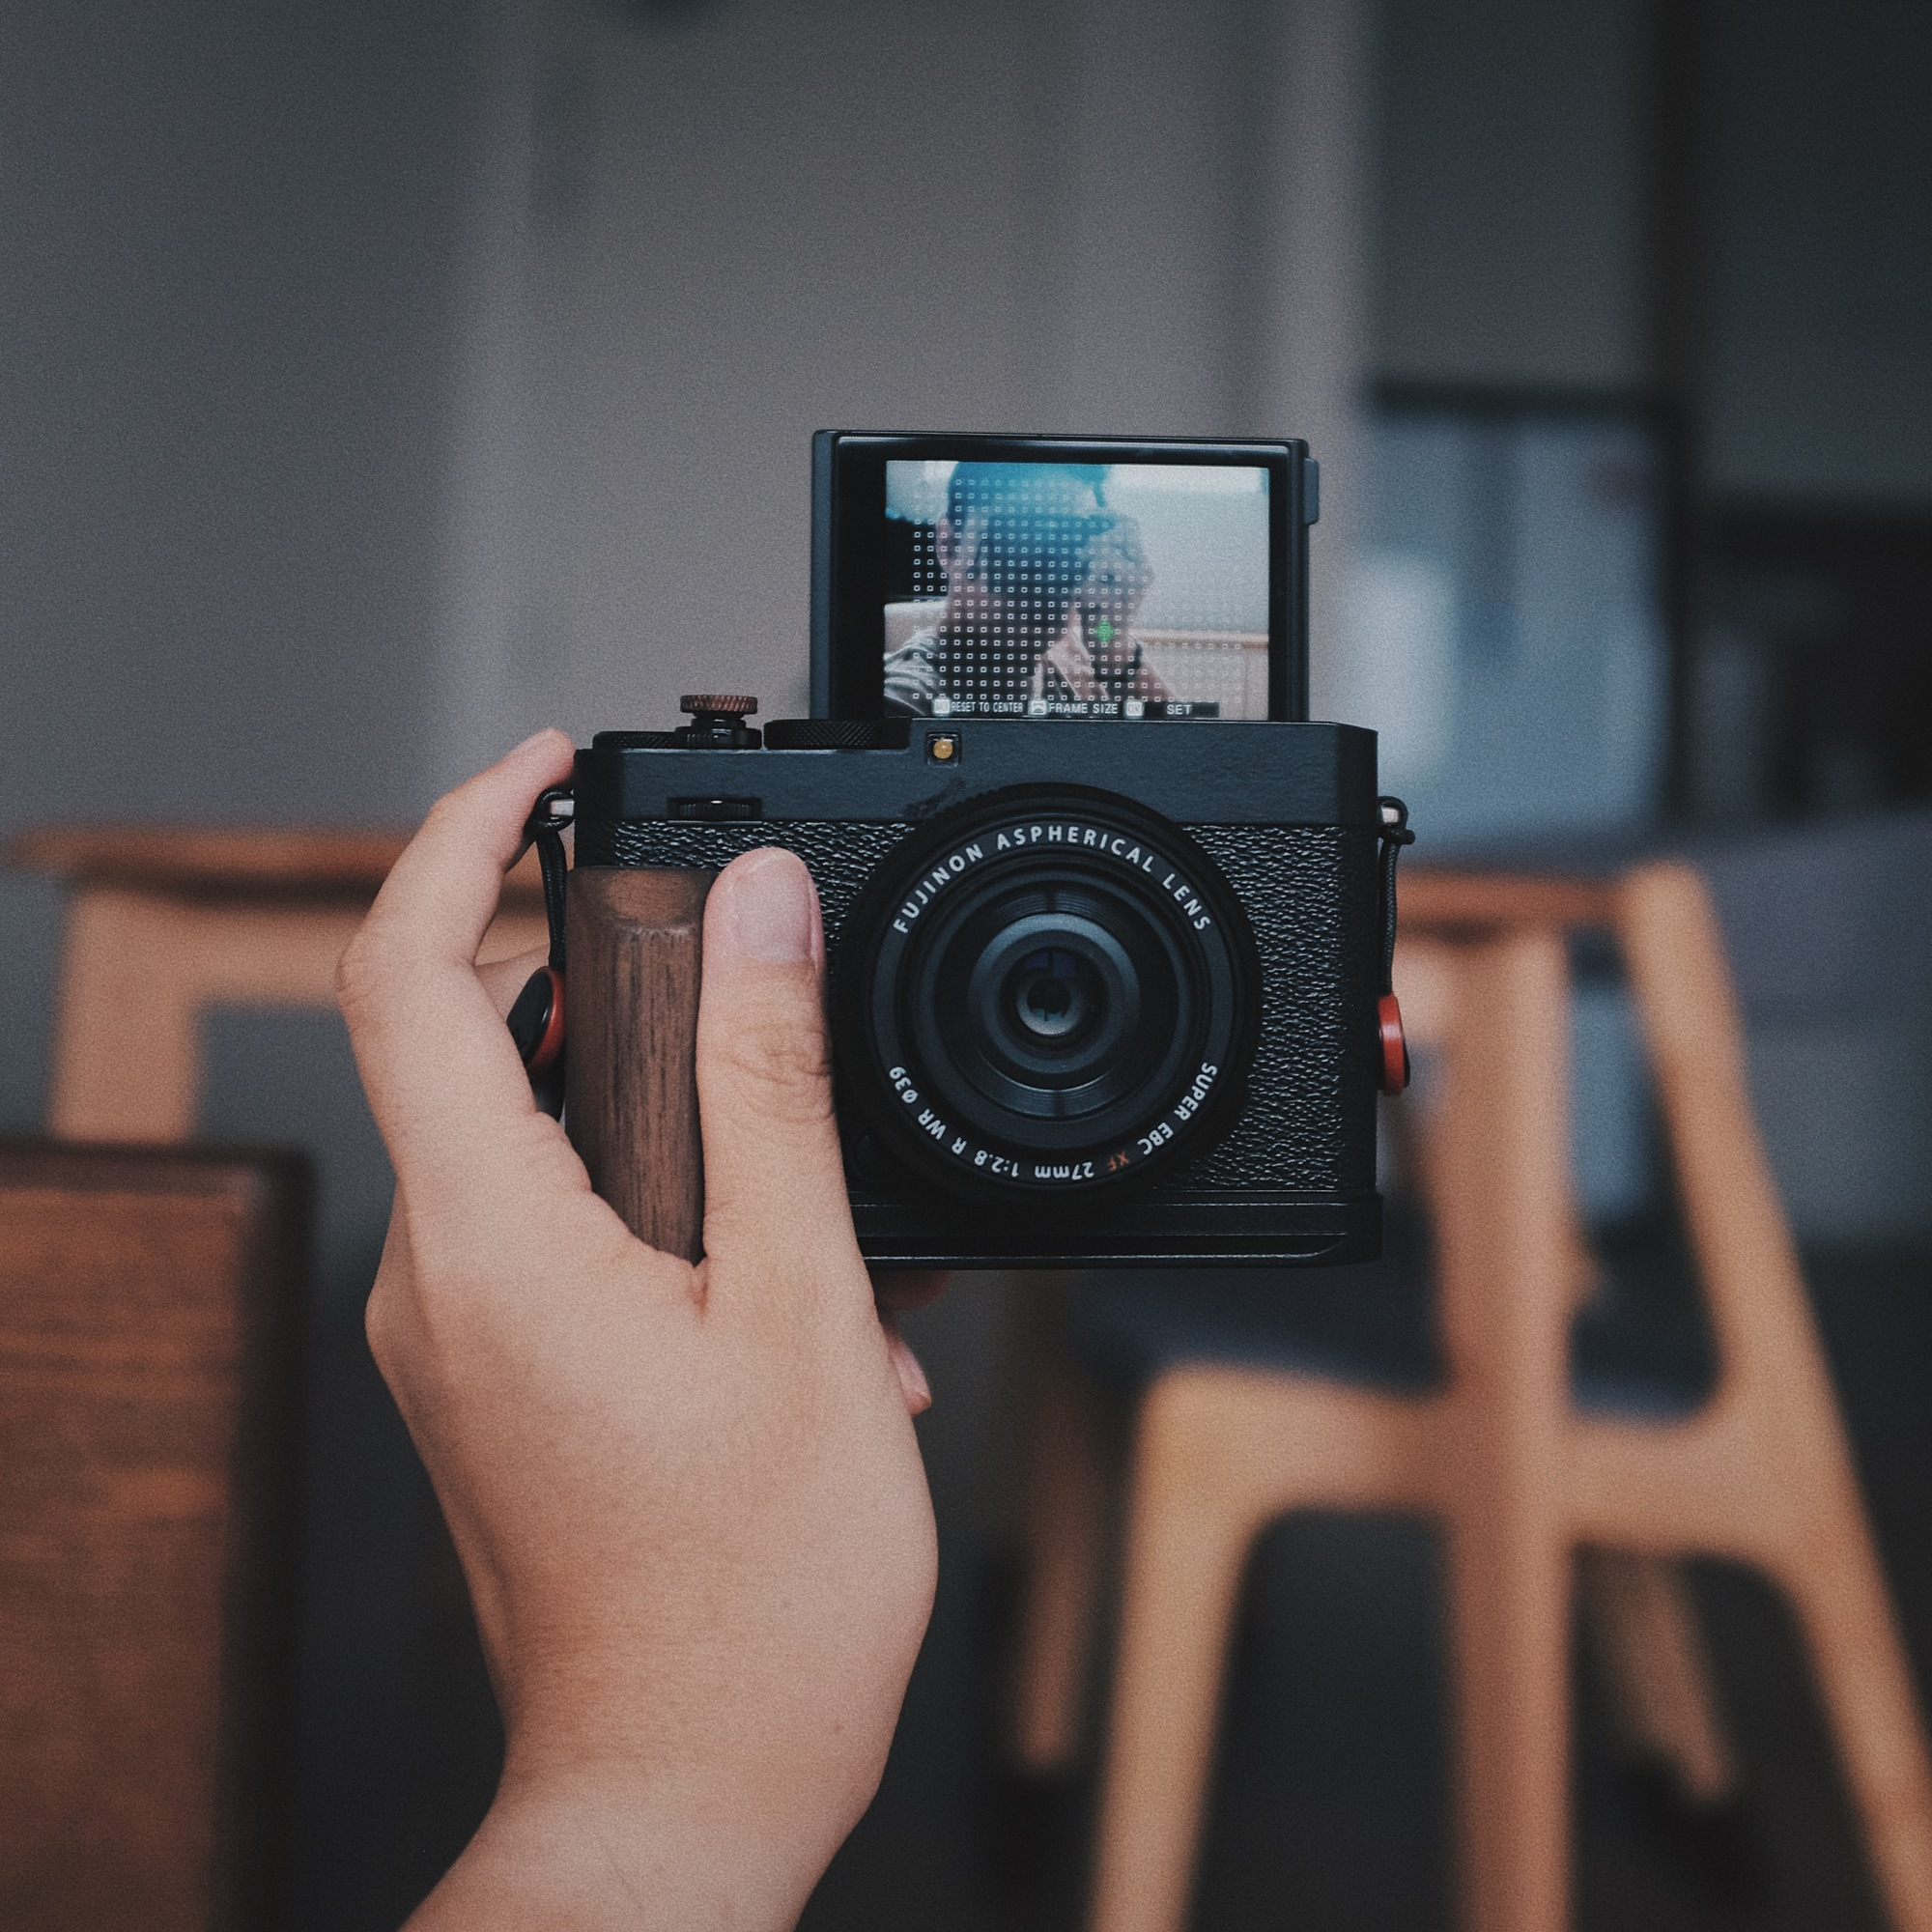
\includegraphics[width=\linewidth]{\envfinaldir/coverpic-prod.jpg}\par
            % \vskip 30pt
            \vfill

            \normalsize\rmfamily\scshape
            \copyright{} The Web Digest Project \hfill\large \envdatestr
        \end{center}
    \end{titlepage}
    % \restoregeometry
}
\newcommand{\simplehref}[1]{%
    \textcolor{blue!80!green}{\href{#1}{#1}}%
}
\renewcommand{\contentsname}{\center\Huge\sffamily\bfseries Contents\par\vskip 20pt}
\newcounter{ipartcounter}
\setcounter{ipartcounter}{0}
\newcommand{\ipart}[1]{
    % \vskip 20pt
    \clearpage
    \stepcounter{ipartcounter}
    \phantomsection
    \addcontentsline{toc}{chapter}{#1}
    % \begin{center}
    %     \Huge
    %     \sffamily\bfseries
    %     #1
    % \end{center}
    % \vskip 20pt plus 7pt
}
\newcounter{ichaptercounter}
\setcounter{ichaptercounter}{0}
\newcommand{\ichapter}[1]{
    % \vskip 20pt
    \clearpage
    \stepcounter{ichaptercounter}
    \phantomsection
    \addcontentsline{toc}{section}{\numberline{\arabic{ichaptercounter}}#1}
    \begin{center}
        \Huge
        \sffamily\bfseries
        #1
    \end{center}
    \vskip 20pt plus 7pt
}
\newcommand{\entrytitlefont}[1]{\subsection*{\raggedright\Large\sffamily\bfseries#1}}
\newcommand{\entryitemGeneric}[2]{
    % argv: title, url
    \parbox{\linewidth}{
        \entrytitlefont{#1}\par\vskip 5pt
        \footnotesize\ttfamily\mdseries
        \simplehref{#2}
    }\vskip 11pt plus 11pt minus 1pt
}
\newcommand{\entryitemGithub}[3]{
    % argv: title, url, desc
    \parbox{\linewidth}{
        \entrytitlefont{#1}\par\vskip 5pt
        \footnotesize\ttfamily\mdseries
        \simplehref{#2}\par\vskip 5pt
        \small\rmfamily\mdseries#3
    }\vskip 11pt plus 11pt minus 1pt
}
\newcommand{\entryitemAp}[3]{
    % argv: title, url, desc
    \parbox{\linewidth}{
        \entrytitlefont{#1}\par\vskip 5pt
        \footnotesize\ttfamily\mdseries
        \simplehref{#2}\par\vskip 5pt
        \small\rmfamily\mdseries#3
    }\vskip 11pt plus 11pt minus 1pt
}
\newcommand{\entryitemHackernews}[3]{
    % argv: title, hnurl, rawurl
    % \parbox{\linewidth}{
    %     \entrytitlefont{#1}\par\vskip 5pt
    %     \footnotesize\ttfamily\mdseries
    %     \simplehref{#3}\par
    %     \textcolor{black!50}{\href{#2}{#2}}
    % }\vskip 11pt plus 11pt minus 1pt
    \begin{minipage}{\linewidth}
            \entrytitlefont{#1}\par\vskip 5pt
            \footnotesize\ttfamily\mdseries
            \simplehref{#3}\par
            \textcolor{black!50}{\href{#2}{#2}}
    \end{minipage}\par\vskip 11pt plus 11pt minus 1pt
}







\begin{document}

\makeheader

\tableofcontents\clearpage




\ipart{Developers}
\ichapter{Hacker News}
\entryitemTwoLinks{Discord hack shows risks of online age checks}{https://news.ycombinator.com/item?id=45551893}{https://news.sky.com/story/discord-hack-shows-dangers-of-online-age-checks-as-internet-policing-hopes-put-to-the-test-13447618}

\entryitemTwoLinks{Microsoft only lets you opt out of AI photo scanning 3x a year}{https://news.ycombinator.com/item?id=45551504}{https://hardware.slashdot.org/story/25/10/11/0238213/microsofts-onedrive-begins-testing-face-recognizing-ai-for-photos-for-some-preview-users}

\entryitemTwoLinks{Rating 26 years of Java changes}{https://news.ycombinator.com/item?id=45551450}{https://neilmadden.blog/2025/09/12/rating-26-years-of-java-changes/}

\entryitemTwoLinks{Tennessee man arrested, accused of threatening a shooting, after posting meme}{https://news.ycombinator.com/item?id=45551352}{https://reason.com/2025/10/10/tennessee-man-arrested-gets-2-million-bond-for-posting-facebook-meme/}

\entryitemTwoLinks{People regret buying Amazon smart displays after being bombarded with ads}{https://news.ycombinator.com/item?id=45551081}{https://arstechnica.com/gadgets/2025/10/people-regret-buying-amazon-smart-displays-after-being-bombarded-with-ads/}

\entryitemTwoLinks{GNU Health}{https://news.ycombinator.com/item?id=45550049}{https://www.gnuhealth.org/about-us.html}

\entryitemTwoLinks{Microsoft Amplifier}{https://news.ycombinator.com/item?id=45549848}{https://github.com/microsoft/amplifier}

\entryitemTwoLinks{Vibing a non-trivial Ghostty feature}{https://news.ycombinator.com/item?id=45549434}{https://mitchellh.com/writing/non-trivial-vibing}

\entryitemTwoLinks{Firefox is the best mobile browser}{https://news.ycombinator.com/item?id=45549308}{https://kelvinjps.com/blog/firefox-best-mobile-browser/}

\entryitemTwoLinks{Learn Turbo Pascal – a video series originally released on VHS}{https://news.ycombinator.com/item?id=45548457}{https://www.youtube.com/watch?v=UOtonwG3DXM}

\entryitemTwoLinks{The <output> Tag}{https://news.ycombinator.com/item?id=45547566}{https://denodell.com/blog/html-best-kept-secret-output-tag}

\entryitemTwoLinks{AV2 video codec delivers 30\% lower bitrate than AV1, final spec due in late 2025}{https://news.ycombinator.com/item?id=45547537}{https://videocardz.com/newz/av2-video-codec-delivers-30-lower-bitrate-than-av1-final-spec-due-in-late-2025}

\entryitemTwoLinks{Daniel Kahneman opted for assisted suicide in Switzerland}{https://news.ycombinator.com/item?id=45547492}{https://www.bluewin.ch/en/entertainment/nobel-prize-winner-opts-for-suicide-in-switzerland-2619460.html}

\entryitemTwoLinks{Windows Subsystem for FreeBSD}{https://news.ycombinator.com/item?id=45547359}{https://github.com/BalajeS/WSL-For-FreeBSD}

\entryitemTwoLinks{Superpowers: How I'm using coding agents in October 2025}{https://news.ycombinator.com/item?id=45547344}{https://blog.fsck.com/2025/10/09/superpowers/}

\entryitemTwoLinks{AMD and Sony's PS6 chipset aims to rethink the current graphics pipeline}{https://news.ycombinator.com/item?id=45546593}{https://arstechnica.com/gaming/2025/10/amd-and-sony-tease-new-chip-architecture-ahead-of-playstation-6/}

\entryitemTwoLinks{Peter Thiel's antichrist lectures reveal more about him than Armageddon}{https://news.ycombinator.com/item?id=45546478}{https://www.theguardian.com/technology/ng-interactive/2025/oct/10/peter-thiel-antichrist-lectures}

\entryitemTwoLinks{How hard do you have to hit a chicken to cook it? (2020)}{https://news.ycombinator.com/item?id=45545965}{https://james-simon.github.io/blog/chicken-cooking/}

\entryitemTwoLinks{Climate goals go up in smoke as US datacenters turn to coal}{https://news.ycombinator.com/item?id=45545277}{https://www.theregister.com/2025/10/10/datacenter\_coal\_power/}

\entryitemTwoLinks{Programming in the Sun: A Year with the Daylight Computer}{https://news.ycombinator.com/item?id=45545098}{https://wickstrom.tech/2025-10-10-programming-in-the-sun-a-year-with-the-daylight-computer.html}\ichapter{Phoronix}
\entryitemGeneric{\hskip 0pt{}Linux 6.18 Lands Retpoline Optimization To Help With Intel E Cores}{https://www.phoronix.com/news/Linux-6.18-Retpoline-Opt}

\entryitemGeneric{\hskip 0pt{}Solus Linux Preparing To Remove Python 2, Big systemd Upgrade \& Finish /usr Merge}{https://www.phoronix.com/news/Solus-Linux-EOY-2025-Epoch}

\entryitemGeneric{\hskip 0pt{}Intel XPU Manager Deprecates Data Center GPU Max Series \& GPU Flex Series}{https://www.phoronix.com/news/Intel-XPU-Manager-1.3.3}

\entryitemGeneric{\hskip 0pt{}Intel Simplifying P-State Driver's Energy Model For Newer Core Ultra CPUs}{https://www.phoronix.com/news/Intel-P-State-Simplify-Energy}

\entryitemGeneric{\hskip 0pt{}Ubuntu 25.10 Fix Pending For Broken Flatpak Support}{https://www.phoronix.com/news/Ubuntu-25.10-Broken-Flatpaks}

\entryitemGeneric{\hskip 0pt{}Phosh 0.50 Released, GNOME App Aims To Help You Learn Assembly}{https://www.phoronix.com/news/Phosh-0.50-Released}

\entryitemGeneric{\hskip 0pt{}KDE Plasma 6.5 Fixing Some Of The Most Common Crashes, Other Bugs Fixed Too}{https://www.phoronix.com/news/Plasma-6.5-Crash-Fixes}

\entryitemGeneric{\hskip 0pt{}Coreboot 25.09 Released With 19 More Motherboards Supported, Better amdfwtool For Turin}{https://www.phoronix.com/news/Coreboot-25.09-Released}

\entryitemGeneric{\hskip 0pt{}Vulkan 1.4.329 Released With New Fused-Multiply Add Extension}{https://www.phoronix.com/news/Vulkan-1.4.329}


\ipart{Developers~~~~(zh-Hans)}
\ichapter{Solidot}
\entryitemGeneric{\hskip 0pt{}小鼠实验显示新癌症疫苗疗效显著}{https://www.solidot.org/story?sid=82521}

\entryitemGeneric{\hskip 0pt{}海关严查英伟达 AI 芯片}{https://www.solidot.org/story?sid=82520}

\entryitemGeneric{\hskip 0pt{}波兰称针对其关键基础设施的网络攻击在增加}{https://www.solidot.org/story?sid=82519}

\entryitemGeneric{\hskip 0pt{}我国成年人日均锌摄入量呈下降趋势}{https://www.solidot.org/story?sid=82518}

\entryitemGeneric{\hskip 0pt{}逾半数富有企业家考虑移民}{https://www.solidot.org/story?sid=82517}

\entryitemGeneric{\hskip 0pt{}ESA 报告称玩家的平均年龄 41 岁}{https://www.solidot.org/story?sid=82516}

\entryitemGeneric{\hskip 0pt{}研究发现让大模型中毒非常容易}{https://www.solidot.org/story?sid=82515}

\entryitemGeneric{\hskip 0pt{}微软开发者披露臭名昭著的 FCKGW 密钥来历}{https://www.solidot.org/story?sid=82514}

\entryitemGeneric{\hskip 0pt{}英特尔重新思考其开源战略}{https://www.solidot.org/story?sid=82513}

\entryitemGeneric{\hskip 0pt{}日全食期间鸟类行为发生改变}{https://www.solidot.org/story?sid=82512}

\entryitemGeneric{\hskip 0pt{}天文学家使用引力透镜发现最小的暗天体}{https://www.solidot.org/story?sid=82511}

\entryitemGeneric{\hskip 0pt{}裸鼹鼠长寿的秘密可能在于其 DNA 修复机制}{https://www.solidot.org/story?sid=82510}

\entryitemGeneric{\hskip 0pt{}GitHub 正将其基础设施迁移到 Azure}{https://www.solidot.org/story?sid=82509}

\entryitemGeneric{\hskip 0pt{}英国央行对 AI 泡沫破裂发出警告}{https://www.solidot.org/story?sid=82508}

\entryitemGeneric{\hskip 0pt{}空客 A320 交付量超过波音 737}{https://www.solidot.org/story?sid=82507}

\entryitemGeneric{\hskip 0pt{}日本公司本月将把酿酒设备送到国际空间站}{https://www.solidot.org/story?sid=82506}

\entryitemGeneric{\hskip 0pt{}DC 漫画称不会支持 AI 创作}{https://www.solidot.org/story?sid=82505}

\entryitemGeneric{\hskip 0pt{}互联网档案馆被命令在比利时屏蔽部分电子书的访问}{https://www.solidot.org/story?sid=82504}

\entryitemGeneric{\hskip 0pt{}Ubuntu 25.10 'Questing Quokka' 释出}{https://www.solidot.org/story?sid=82503}

\entryitemGeneric{\hskip 0pt{}黄金价格首次突破每盎司 4000 美元}{https://www.solidot.org/story?sid=82502}\ichapter{V2EX}
\entryitemGeneric{\hskip 0pt{}[生活] 盘点以下我用坏的小米产品}{https://www.v2ex.com/t/1164584}

\entryitemGeneric{\hskip 0pt{}[推广] 科普|``ChatGPT 卡密自助充值站''1 分钟免登录自动化订阅 PLUS?别再交出你的 ChatGPT 登录认证 token 了}{https://www.v2ex.com/t/1164579}

\entryitemGeneric{\hskip 0pt{}[反馈] 可能是论坛的一个 BUG?}{https://www.v2ex.com/t/1164577}

\entryitemGeneric{\hskip 0pt{}[职场话题] 两轮技术面试过后突然加了一轮面试,这是什么意思}{https://www.v2ex.com/t/1164576}

\entryitemGeneric{\hskip 0pt{}[职场话题] 工作两年了,思考和迷茫}{https://www.v2ex.com/t/1164575}

\entryitemGeneric{\hskip 0pt{}[随想] 2021 年失业后,在 2022 年我把房贷还清,到今年累计赚到新的一百万。}{https://www.v2ex.com/t/1164574}

\entryitemGeneric{\hskip 0pt{}[问与答] 安卓手机现在推荐什么}{https://www.v2ex.com/t/1164573}

\entryitemGeneric{\hskip 0pt{}[问与答] Cursor 最近变得快用不起了}{https://www.v2ex.com/t/1164571}

\entryitemGeneric{\hskip 0pt{}[分享发现] google 翻译会把一些不清楚的人名翻译成著名人物,qian,wen}{https://www.v2ex.com/t/1164570}

\entryitemGeneric{\hskip 0pt{}[Solana] BTC 四年周期被打破了嘛?}{https://www.v2ex.com/t/1164568}

\entryitemGeneric{\hskip 0pt{}[程序员] Claude Code 无法访问文件?}{https://www.v2ex.com/t/1164567}

\entryitemGeneric{\hskip 0pt{}[问与答] Windows 微信来电的时候会导致游戏弹出到桌面,如何设置才能让微信来电的时候不弹出到桌面?}{https://www.v2ex.com/t/1164565}

\entryitemGeneric{\hskip 0pt{}[DNS] 如何排查自建 DNS 中的问题?}{https://www.v2ex.com/t/1164563}

\entryitemGeneric{\hskip 0pt{}[酷工作] 招聘: Position 一: Quant Trader / Desk Quant Position 二: DevRel Engineer Position 三: APAC Community Lead}{https://www.v2ex.com/t/1164562}

\entryitemGeneric{\hskip 0pt{}[Apple TV] 最近 TV+ 直连速度很慢,有合适的 DNS 可以改善吗?}{https://www.v2ex.com/t/1164561}

\entryitemGeneric{\hskip 0pt{}[VPS] 低价的 Windows VPS(主要 RDP 远程桌面)}{https://www.v2ex.com/t/1164560}

\entryitemGeneric{\hskip 0pt{}[分享发现] 发现 RARBG 压制的影片真的好}{https://www.v2ex.com/t/1164559}

\entryitemGeneric{\hskip 0pt{}[Solana] 应 @carson8899 大佬需求, 录制了一个 web 钱包关联和手机钱包关联的视频,给需要的新绑定用户参考.}{https://www.v2ex.com/t/1164558}

\entryitemGeneric{\hskip 0pt{}[职场话题] 领英沟通中突然消息消失了}{https://www.v2ex.com/t/1164557}

\entryitemGeneric{\hskip 0pt{}[Solana] OKX 连接 V2EX 账户指南}{https://www.v2ex.com/t/1164555}

\entryitemGeneric{\hskip 0pt{}[Linux] Debian 12 下 i9-14900HX Turbo Boost 被异常禁用,无法手动启用}{https://www.v2ex.com/t/1164554}

\entryitemGeneric{\hskip 0pt{}[问与答] 浙江流量卡推荐}{https://www.v2ex.com/t/1164553}

\entryitemGeneric{\hskip 0pt{}[macOS] macos 如何将应用安装到外置硬盘}{https://www.v2ex.com/t/1164551}

\entryitemGeneric{\hskip 0pt{}[macOS] mac 投屏到 iPad 上}{https://www.v2ex.com/t/1164550}

\entryitemGeneric{\hskip 0pt{}[职场话题] 创业有感,对流量的另一种认知}{https://www.v2ex.com/t/1164549}

\entryitemGeneric{\hskip 0pt{}[问与答] 抽烟的人闻不到味道吗?}{https://www.v2ex.com/t/1164548}

\entryitemGeneric{\hskip 0pt{}[Apple] 国产手机拍照已经秒杀 iPhone 了,系统流畅度也跟上了,为什么还是选择 iPhone}{https://www.v2ex.com/t/1164547}

\entryitemGeneric{\hskip 0pt{}[程序员] 正在创建一个产品共创红包群,欢迎加入}{https://www.v2ex.com/t/1164546}

\entryitemGeneric{\hskip 0pt{}[电动汽车] 告特斯拉,告赢了。}{https://www.v2ex.com/t/1164545}

\entryitemGeneric{\hskip 0pt{}[宽带症候群] 为了避免被运营商骚扰,各位 PTer 有什么专门的设置么?}{https://www.v2ex.com/t/1164544}

\entryitemGeneric{\hskip 0pt{}[macOS] Mac 解压问题}{https://www.v2ex.com/t/1164542}

\entryitemGeneric{\hskip 0pt{}[Apple] 牛马工具合影。}{https://www.v2ex.com/t/1164541}

\entryitemGeneric{\hskip 0pt{}[问与答] 帮 Vtuber 樱花妹求救一下}{https://www.v2ex.com/t/1164540}

\entryitemGeneric{\hskip 0pt{}[分享发现] 没错,就是硬广!超清无水印版 Sora2,可以试用!}{https://www.v2ex.com/t/1164538}

\entryitemGeneric{\hskip 0pt{}[分享创造] [免费无广无内购] SavePoint - 时间机器太重?试试这个轻量级 macOS 文件快照管理工具!}{https://www.v2ex.com/t/1164537}

\entryitemGeneric{\hskip 0pt{}[Apple] iOS26 截图后小窗经常不出现}{https://www.v2ex.com/t/1164536}

\entryitemGeneric{\hskip 0pt{}[程序员] MoonBit 编程语言添加异步支持功能,能用来做什么?}{https://www.v2ex.com/t/1164533}

\entryitemGeneric{\hskip 0pt{}[Solana] 特朗普发布关税消息 30 分钟前开了一个比特币空头,现在赚了 8800 万美元,猜猜是谁?}{https://www.v2ex.com/t/1164531}

\entryitemGeneric{\hskip 0pt{}[NAS] 群晖 DS920 重组存储,求推荐 M.2/2280/4T}{https://www.v2ex.com/t/1164530}

\entryitemGeneric{\hskip 0pt{}[加密货币] 做了一个币安 Alpha 新币推送的站点,欢迎大家体验。}{https://www.v2ex.com/t/1164528}

\entryitemGeneric{\hskip 0pt{}[酷工作] AI 初创公司,南宁寻全栈工程师}{https://www.v2ex.com/t/1164527}

\entryitemGeneric{\hskip 0pt{}[酷工作] Java 后端内推(中-高级), Base 深圳高新园,强度有点高,总包可以}{https://www.v2ex.com/t/1164526}

\entryitemGeneric{\hskip 0pt{}[程序员] 还有啥 AI 方向可以做的业务不 讨论讨论~}{https://www.v2ex.com/t/1164525}

\entryitemGeneric{\hskip 0pt{}[Apple] 请教一个家庭里彻底清除 Homepod Mini 残留的问题}{https://www.v2ex.com/t/1164524}

\entryitemGeneric{\hskip 0pt{}[酷工作] [重庆渝北 8-11K] 海外电商公司招聘前端 2 名}{https://www.v2ex.com/t/1164523}

\entryitemGeneric{\hskip 0pt{}[问与答] 闪电贷贷了一笔款,想用于公司投资,应该怎么操作?}{https://www.v2ex.com/t/1164522}

\entryitemGeneric{\hskip 0pt{}[问与答] B 站上的大流量卡是真的吗}{https://www.v2ex.com/t/1164521}

\entryitemGeneric{\hskip 0pt{}[生活] 体检结果出来了,真得戒烟戒酒了}{https://www.v2ex.com/t/1164520}

\entryitemGeneric{\hskip 0pt{}[生活] 国庆参加了一个高中同学聚会}{https://www.v2ex.com/t/1164519}

\entryitemGeneric{\hskip 0pt{}[C++] 使用匿名结构体指针作为常量来杜绝魔数,是否合理/值得?}{https://www.v2ex.com/t/1164518}


\ipart{Generic News}







\clearpage
\leavevmode\vfill
\footnotesize

Copyright \copyright{} 2023-2025 Neruthes and other contributors.

This document is published with CC BY-NC-ND 4.0 license.

The entries listed in this newsletter may be copyrighted by their respective creators.

This newsletter is generated by the Web Digest project.

The newsletters are also delivered via Telegram channel \CJKunderline{\href{https://t.me/webdigestchannel}{https://t.me/webdigestchannel}}.\\
RSS feed is available at \CJKunderline{\href{https://webdigest.pages.dev/rss.xml}{https://webdigest.pages.dev/rss.xml}}.

This newsletter is available in PDF at
\CJKunderline{\href{https://webdigest.pages.dev/}{https://webdigest.pages.dev/}}.

The source code being used to generate this newsletter is available at\\
\CJKunderline{\href{https://github.com/neruthes/webdigest}{https://github.com/neruthes/webdigest}}.

This newsletter is also available in
\CJKunderline{\href{http://webdigest.pages.dev/readhtml/\envyear/WebDigest-20251012.html}{HTML}} and
\CJKunderline{\href{https://github.com/neruthes/webdigest/blob/master/markdown/\envyear/WebDigest-20251012.md}{Markdown}}.


\coverpic{https://unsplash.com/photos/a-tall-glass-of-golden-beer-with-foam-imfa6ckaduo}{Robert | Visual Diary | Berlin}


\end{document}
